% !TEX root = ../supp.tex
\begin{figure}[t]
\centering
% \vspace{-0.2in}
\iflatexml
    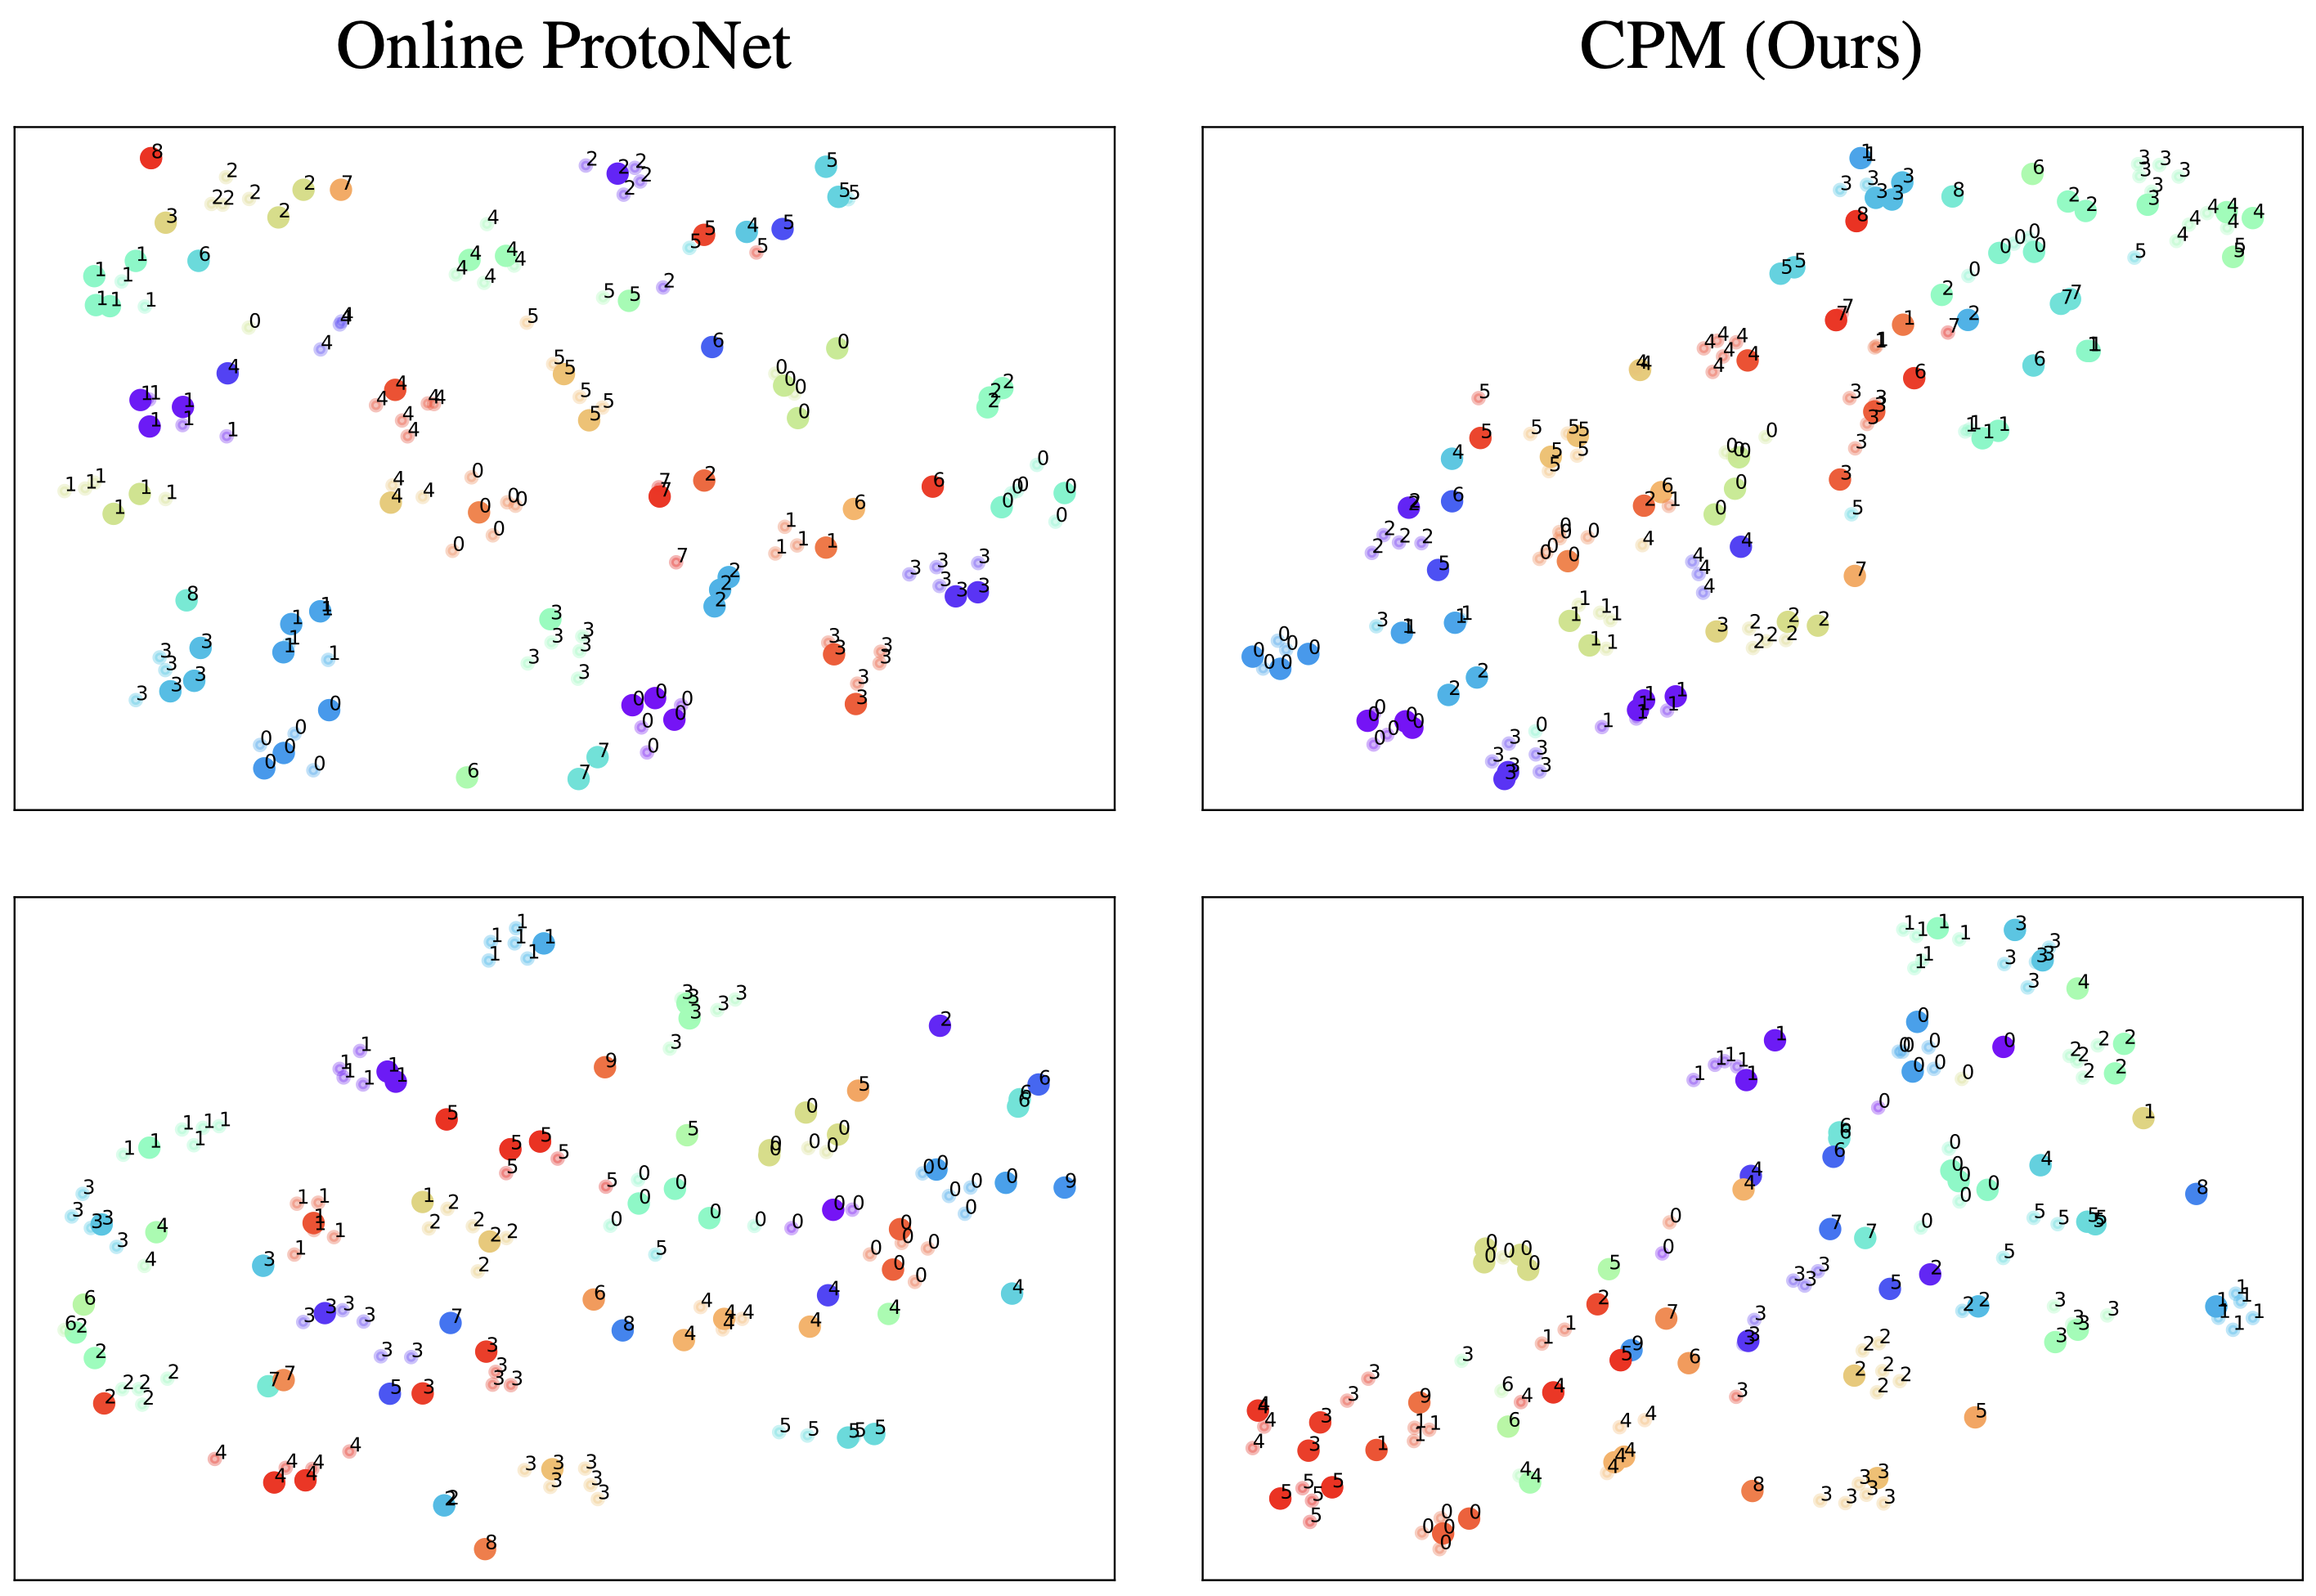
\includegraphics[width=6\linewidth]{figures/omniglot-tsne.png}
\else
    \begin{tabular}{cc}
    Online ProtoNet & CPM (Ours) \\
    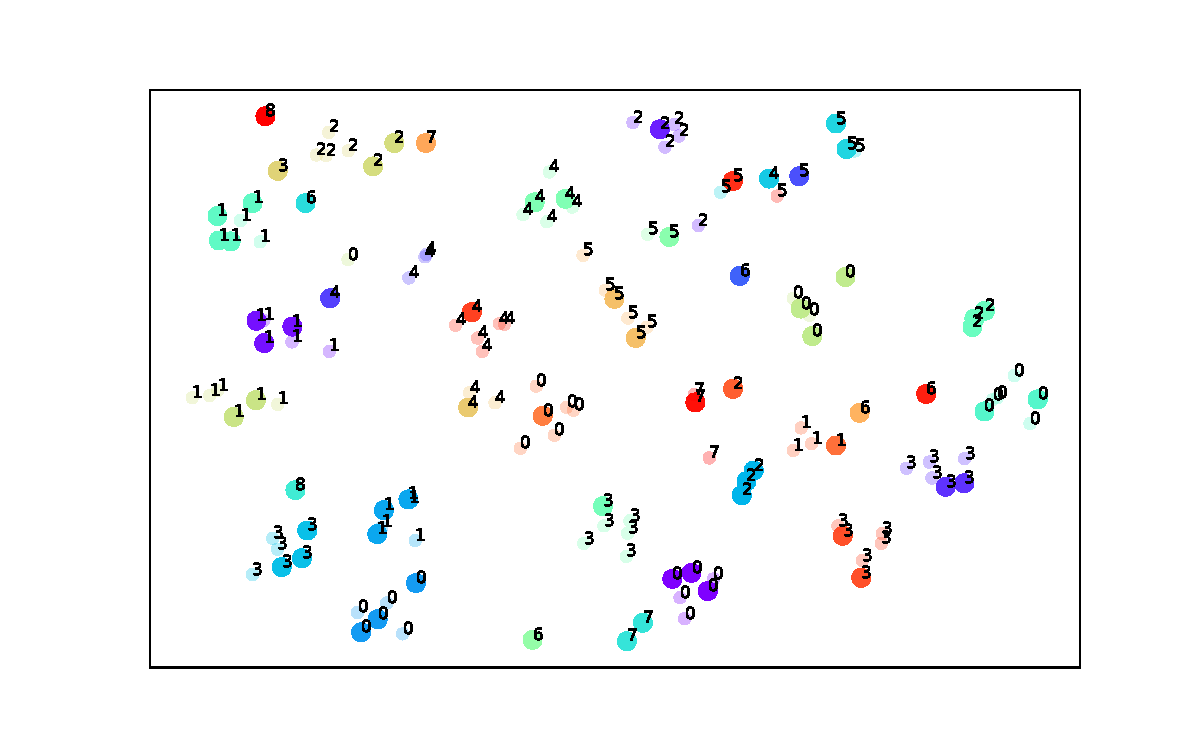
\includegraphics[height=3.8cm, trim={2.5cm 1cm 2cm 1cm}, clip]{figures/omniglot-protonet-tsne/tsne-003.pdf}
    &
    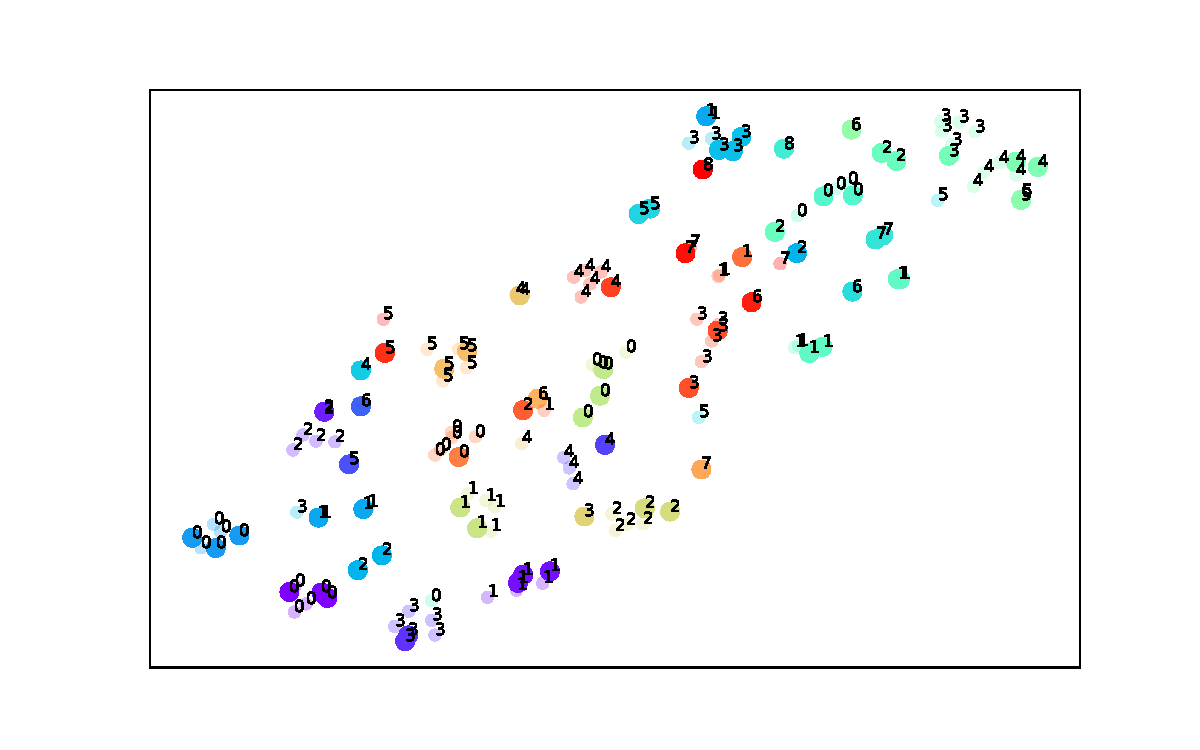
\includegraphics[height=3.8cm, trim={2.5cm 1cm 2cm 1cm}, clip]{figures/omniglot-cpm-tsne/tsne-003.pdf}
    \\
    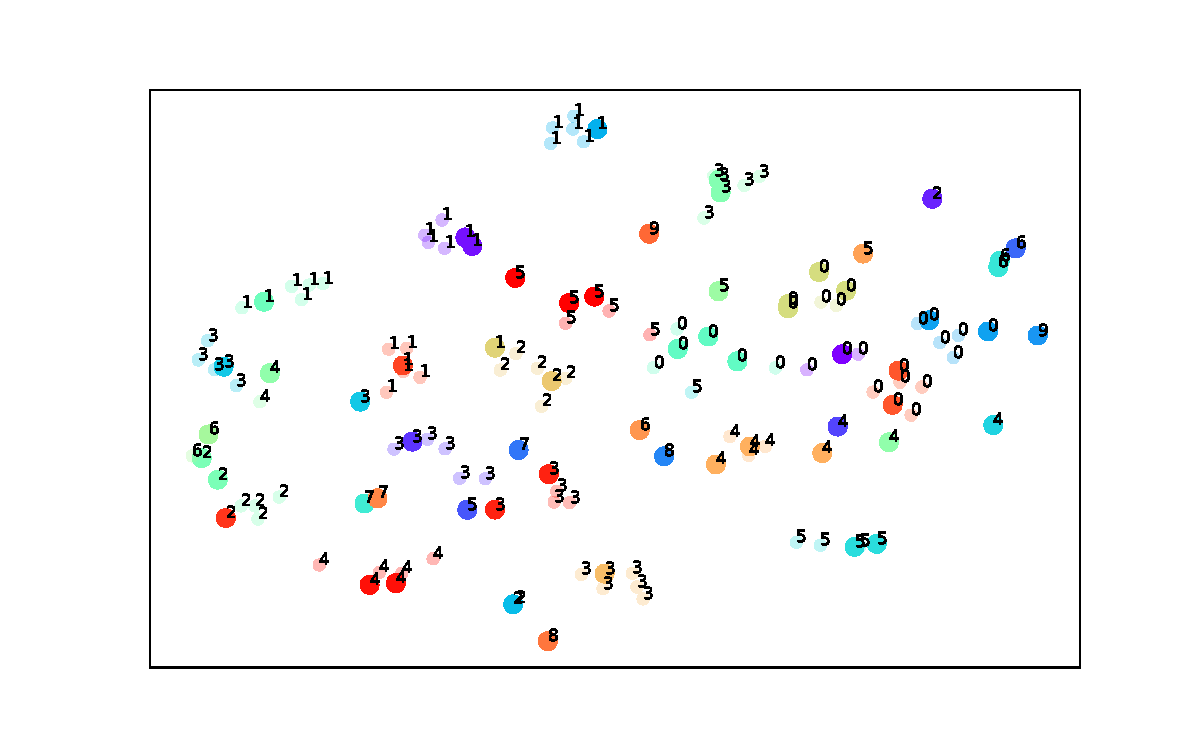
\includegraphics[height=3.8cm, trim={2.5cm 1cm 2cm 1cm}, clip]{figures/omniglot-protonet-tsne/tsne-008.pdf}
    &
    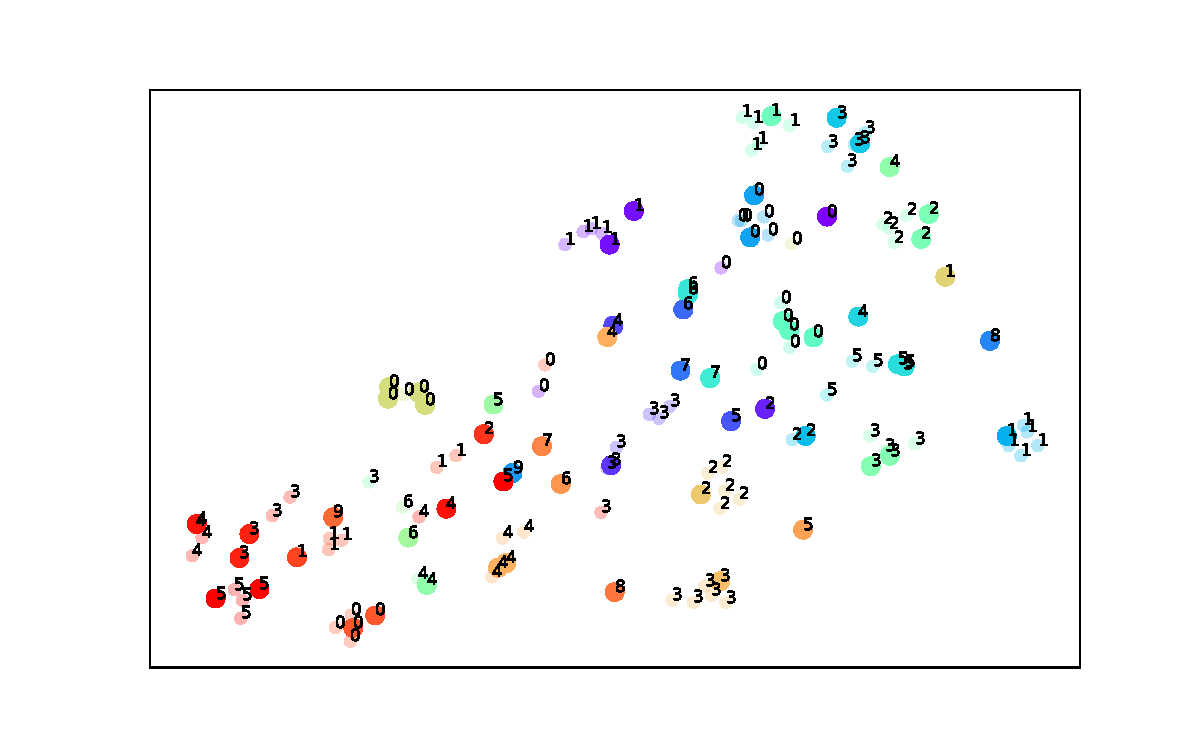
\includegraphics[height=3.8cm, trim={2.5cm 1cm 2cm 1cm}, clip]{figures/omniglot-cpm-tsne/tsne-008.pdf}
    \end{tabular}
\fi
\caption{\textbf{Embedding space visualization of \ourchar{} sequences using t-SNE~\citep{tsne}}. Different color
denotes different environments. Text labels (relative to each environment) are annotated beside the
scatter points. Unlabeled examples shown in smaller circles with lighter colors. \textbf{Left:}
Online ProtoNet; \textbf{Right:} CPM. The embeddings learned CPM model shows a smoother transition
of classes based on their temporal environments.}
\label{fig:tsne}
\end{figure}
